\documentclass[a4paper]{article}

\usepackage[pages=all, color=black, position={current page.south}, placement=bottom, scale=1, opacity=1, vshift=5mm]{background}
\usepackage[margin=1in]{geometry} % full-width

% AMS Packages
\usepackage{amsmath}
\usepackage{amsthm}
\usepackage{amssymb}

% Unicode
\usepackage[utf8]{inputenc}
\usepackage{hyperref}
\hypersetup{
    unicode,
%   colorlinks,
%   breaklinks,
%   urlcolor=cyan, 
%   linkcolor=blue, 
    pdfauthor={Author One, Author Two, Author Three},
    pdftitle={A simple article template},
    pdfsubject={A simple article template},
    pdfkeywords={article, template, simple},
    pdfproducer={LaTeX},
    pdfcreator={pdflatex}
}

% Natbib
\usepackage[sort&compress,numbers,square]{natbib}
\bibliographystyle{mplainnat}

% Theorem, Lemma, etc
\theoremstyle{plain}
\newtheorem{theorem}{Theorem}
\newtheorem{corollary}[theorem]{Corollary}
\newtheorem{lemma}[theorem]{Lemma}
\newtheorem{claim}{Claim}[theorem]
\newtheorem{axiom}[theorem]{Axiom}
\newtheorem{conjecture}[theorem]{Conjecture}
\newtheorem{fact}[theorem]{Fact}
\newtheorem{hypothesis}[theorem]{Hypothesis}
\newtheorem{assumption}[theorem]{Assumption}
\newtheorem{proposition}[theorem]{Proposition}
\newtheorem{criterion}[theorem]{Criterion}
\theoremstyle{definition}
\newtheorem{definition}[theorem]{Definition}
\newtheorem{example}[theorem]{Example}
\newtheorem{remark}[theorem]{Remark}
\newtheorem{problem}[theorem]{Problem}
\newtheorem{principle}[theorem]{Principle}

\usepackage{graphicx, color}
\graphicspath{{fig/}}

%\usepackage[linesnumbered,ruled,vlined,commentsnumbered]{algorithm2e} % use algorithm2e for typesetting algorithms
\usepackage{algorithm, algpseudocode} % use algorithm and algorithmicx for typesetting algorithms
\usepackage{mathrsfs} % for \mathscr command

\usepackage{lipsum}

% Author info
\title{Multi-Model Movie Recommendation System}
\author{
    Aansh Dubey (B22AI058) \\
    Aditya Padhy (B22ES005)\\
    Advait Gaur (B22CS004) \\
    Aniket Singh (B22CS009) \\
    Qazi Talha Ali (B22CS087) \\
}


% \date{
%     $^1$Organization 1 \\ \texttt{\{auth1, auth3\}@org1.edu}\\%
%     $^2$Organization 2 \\ \texttt{auth3@inst2.edu}\\[2ex]%
% %   \today
% }

% % Background and color
% \definecolor{orangeaccent2lighter40}{RGB}{242,213,177}
% \backgroundsetup{
% scale=1,
% angle=0,
% opacity=1,
% contents={\begin{tikzpicture}[remember picture,overlay]
% \node at (current page.center) {\includegraphics[width=\paperwidth,height=\paperheight]{example-image}};
% \end{tikzpicture}}
% }

\begin{document}
    \maketitle
    
    \begin{abstract}
        This article presents a simple movie recommendation system developed using the MovieLens dataset. The system incorporates collaborative filtering, content-based filtering, hybrid filtering, Naive Bayes approach, and logistic regression approach to generate personalized movie recommendations for users. The experimental results demonstrate the effectiveness of the proposed system in providing accurate and diverse movie recommendations.\\ \\
            
        \noindent\textbf{Keywords:} movie recommendation, collaborative filtering, content-based filtering, hybrid filtering, Naive Bayes, logistic regression
        \vspace{15cm}
    \end{abstract}

    \tableofcontents

\section{Introduction}
\label{sec:intro}
The aim of this project is to develop a Movie Recommendation System, based on the Movie Lens Small Latest Dataset. The objective is to develop a model that recommends movies based on either the user or a particular movie.\\
We will test the following models to find the best approach to Movie Recommendation.

\subsection*{Collaborative Filtering}

The collaborative filtering approach is a fundamental method used in recommendation systems. It works on the assumption that users who have agreed in the past tend to agree again in the future. By identifying similarities between users or items based on their interactions, collaborative filtering generates recommendations by leveraging the collective preferences of similar users or items.

\subsection*{Content-Based Filtering}
Content-based filtering recommends items based on their attributes and features. In the context of movie recommendation systems, this approach analyzes movie characteristics such as genre, cast, director, and plot summary. By identifying similarities between movies based on these attributes, content-based filtering suggests movies that are similar to those that a user has liked in the past.

\subsection*{Hybrid Filtering}
Hybrid filtering combines collaborative filtering and content-based filtering techniques to enhance recommendation accuracy. By leveraging the strengths of both approaches, hybrid filtering mitigates their individual weaknesses. This approach integrates user preferences, item attributes, and collaborative interactions to provide more accurate and diverse recommendations tailored to individual users' preferences and interests.


\subsection*{Naive Bayes Approach}
Naive Bayes Approach:
The Naive Bayes approach aims to develop a movie genre classification system and recommendation system using the MovieLens dataset. Leveraging the principles of Naive Bayes classifiers, this approach focuses on predicting movie genres based on user ratings and preferences. By analyzing user interactions and movie attributes, the system aims to recommend movies that align closely with the user's interests and preferences.

\subsection*{Logistic Regression Approach}
The Logistic Regression approach also aims to create a movie genre classification system and recommendation system using the MovieLens dataset. Unlike the Naive Bayes approach, Logistic Regression focuses on predicting user ratings for movies based on their genre attributes. By training individual logistic regression models for each user, the system predicts the likelihood of a user enjoying a particular movie genre, thereby facilitating personalized movie recommendations.

\section{Model Description}

\subsection{Collaborative Filtering}

    \textbf{Assumption:} If a user A likes certain items and a user B shares similar preferences with user A, then user A is likely to also like items that user B likes. Thus, our main priority is to find the “similarity” between two users.\\

    \textbf{Method:} Find similar movies based on user-item interactions using k-nearest neighbors (kNN). Similarity is typically measured using metrics like cosine similarity, which calculates the cosine of the angle between two vectors (user vectors in this case).\\

    \textbf{Problem:} There exist movies with abnormally low ratings, which may skew their ratings.\\

    \textbf{Solution:} Calculate the Bayesian average ratings for each movie to mitigate the effect of movies with very few ratings.\\

    \textbf{Bayesian Average Ratings:}

    Bayesian Average is a statistical method used to calculate the weighted average of ratings, which takes into account not only the raw average rating but also the number of ratings each item has received. It's particularly useful in scenarios where some items have very few ratings, as it helps to stabilize the ratings by incorporating a prior assumption about the data.\\

    \textbf{Algorithm to calculate Bayesian Average ratings mathematically:}

        \begin{enumerate}
            \item \textbf{Define Variables:}
            \begin{itemize}
                \item \( C \): The average number of ratings for a given item (movie in this case).
                \item \( m \): The average rating for a given item.
            \end{itemize}
            \item \textbf{Calculate Bayesian Average:}
            For each item (movie), the Bayesian Average is computed using the formula:
            \[
            \text{Bayesian Average} = \frac{{C \cdot m + \sum \text{of Ratings}}}{{C + \text{number of ratings}}}
            \]
            Where:
            \begin{itemize}
                \item \( C \cdot m \): Represents the prior assumption about the data. It's the product of the average number of ratings per item and the overall average rating. This serves as a baseline expectation for the rating.
                \item \( \sum \text{of Ratings} \): The sum of all ratings for the item.
                \item \( C + \text{number of ratings} \): The total number of ratings for the item, including the prior assumption (C) and the actual ratings.
            \end{itemize}
        \end{enumerate}
        
        \textbf{Example:} Let's say we have a movie with the following ratings:
        \begin{itemize}
            \item Average rating for all movies (\( m \)): 3.8
            \item Average number of ratings per movie (\( C \)): 40
            \item Number of ratings for the movie: 20
            \item Sum of ratings for the movie: 60
        \end{itemize}
        Using the formula, the Bayesian Average would be calculated as follows:
        \[
        \text{Bayesian Average} = \frac{{40 \times 3.8 + 60}}{{40 + 20}} = \frac{{152 + 60}}{{60}} \approx 3.533
        \]
        
        In this example, the Bayesian Average for the movie is approximately 3.533. The original rating for this movie is \( \frac{{60}}{{20}} = 3 \). We can compare this to the Bayesian Average:
        \begin{itemize}
            \item Original Rating: 3
            \item Bayesian Average: 3.533
        \end{itemize}
        In this example, the original rating (3) differs from the Bayesian Average (3.533). This difference indicates that the Bayesian Average has adjusted the rating based on the prior assumption (average rating for all movies) and the number of ratings received by the movie. The Bayesian Average provides a more stable estimate that takes into account the overall distribution of ratings and the number of ratings for the specific movie, which can be particularly useful when dealing with sparse or biased datasets.
        
        \textbf{Hyperparameters:} 
        \begin{itemize}
            \item No. of suggestions: 200
        \end{itemize}


    \subsection{Content-Based Filtering}

        \textbf{Line of Thought:} User will be interested in movies similar to those the user has liked in the past. Thus, we focus on finding the “similarity” between two users. It computes the similarity between movies based on their genre attributes using \textbf{cosine similarity}.\\
        
        \textbf{Approach :}
        \begin{enumerate}
            \item \textbf{Step 1: Extracting Unique Genres:}
            Creates a set of unique genres present in the \textbf{genres} column of the \textbf{movie\_df} DataFrame by using \textbf{set} function and iterating over each row of the \textbf{genres} column (G) and then iterating over each genre (\textbf{g}) within that row.
            
            \item \textbf{Step 2: Creating Binary Genre Columns:}
            For each genre (\textbf{g}), we create a new binary column in the \textbf{movie\_df} DataFrame. Each movie is assigned a \textbf{1} if it belongs to the current genre \textbf{g}, and \textbf{0} otherwise.

            
            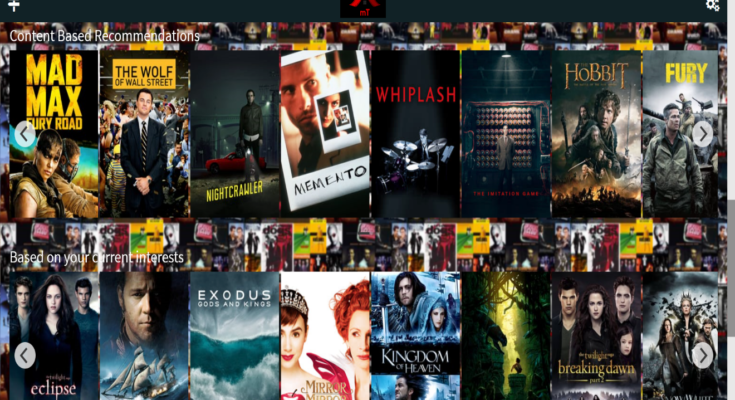
\includegraphics[width=\linewidth, height=3cm]{image1.png} % Include your image here with increased height
            
            \item \textbf{Step 3: Creating Movie Genres DataFrame:}
            Create new DataFrame \textbf{movie\_genres} with only the binary genre columns, where each row represents a movie and each column represents a genre.
            
            \item \textbf{Step 4: Computing Cosine Similarity:}
            Using the \textbf{sklearn}’s \textbf{cosine\_similarity} function, we compute the cosine similarity between the \textbf{movie\_genres} DataFrame and itself. This calculates the pairwise cosine similarity between each pair of movies based on their binary genre representations. Each entry (i, j) represents the cosine similarity between movie \textbf{i} and movie \textbf{j} based on their genre attributes.

            \includegraphics[width=\linewidth, height=3cm]{image2.png} % Include your image here with increased height
            
            \item \textbf{Step 5: Creating Movie Index Dictionary:}
            We create a dictionary named \textbf{movie\_idx} using the \textbf{zip} function, which maps movie IDs to their corresponding indices in the \textbf{movie\_df} DataFrame. This allows us to easily retrieve the index of a movie given its ID.
            
            \item \textbf{Step 6: Retrieving Movie Index:}
            We retrieve the index of a specific movie (\textbf{movie\_id}) from the \textbf{movie\_idx} dictionary. This index corresponds to the row index of the movie in the \textbf{movie\_genres} DataFrame, and print the index along with its title and ID.\\
        \end{enumerate}
        
        % \textbf{Example Recommendation:}
        % \begin{itemize}
        %     \item Suppose a user has watched \textbf{"Toy Story (1995)"} with genres \textbf{"Adventure|Animation|Children|Comedy|Fantasy"}.
        %     \item The content-based filtering system would find other movies with similar genre combinations, such as \textbf{"Jumanji (1995)"} with genres \textbf{"Adventure|Children|Fantasy"}.
        %     \item It might also consider recommending movies like \textbf{"Shrek (2001)"} with genres \textbf{"Adventure|Animation|Children|Comedy|Fantasy"}, as it shares similar genre attributes with \textbf{"Toy Story"}.
        % \end{itemize}

            \textbf{Example Calculation of Cosine Similarity:}
            \\
            Suppose we have a set of users with their corresponding ratings for a set of movies as follows:
            
            \begin{center}
            \begin{tabular}{|c|c|c|c|}
            \hline
            \textbf{User ID} & \textbf{Movie 1 (ID)} & \textbf{Movie 2 (ID)} & \textbf{Movie 3 (ID)} \\
            \hline
            1 & 5 & 4 & 0 \\
            2 & 0 & 5 & 3 \\
            3 & 4 & 0 & 0 \\
            \hline
            \end{tabular}
            \end{center}
            
            We want to compute the cosine similarity between each pair of users based on their movie ratings.
            
            The cosine similarity between two users $i$ and $j$ is calculated using the formula:
            
            \[
            \text{similarity}(i, j) = \frac{{\text{dot product of rating vectors }(i, j)}}{{\text{magnitude of rating vector }i \times \text{magnitude of rating vector }j}}
            \]
            
            Let's compute the cosine similarity between users 1 and 2 as an example:
            
            \begin{enumerate}
                \item \textbf{Dot Product of Rating Vectors (1, 2):}
                \[
                \text{Dot Product} = (5 \times 0) + (4 \times 5) + (0 \times 3) = 0 + 20 + 0 = 20
                \]
                
                \item \textbf{Magnitude of Rating Vector 1 ($\|1\|$):}
                \[
                \|1\| = \sqrt{(5^2 + 4^2 + 0^2)} = \sqrt{25 + 16 + 0} = \sqrt{41}
                \]
                
                \item \textbf{Magnitude of Rating Vector 2 ($\|2\|$):}
                \[
                \|2\| = \sqrt{(0^2 + 5^2 + 3^2)} = \sqrt{0 + 25 + 9} = \sqrt{34}
                \]
                
                \item \textbf{Cosine Similarity between Users 1 and 2:}
                \[
                \text{Similarity}(1, 2) = \frac{20}{{\sqrt{41} \times \sqrt{34}}} \approx \frac{20}{\sqrt{1394}} \approx 0.492
                \]
            \end{enumerate}
            
            So, the cosine similarity between users 1 and 2 is approximately 0.492.
            
            Similarly, cosine similarities can be computed for other pairs of users in the dataset.


    \subsection{Hybrid Filtering}

        \textbf{Idea:}
        Hybrid filtering combines collaborative and content-based filtering to improve recommendation accuracy. It leverages the strengths of both approaches and mitigates their weaknesses.
        
        \textbf{Method:}
        
        \begin{enumerate}
            \item \textbf{Step 1: Retrieving Movie Title:}
            
            We retrieve the index of the input movie (\textit{movie\_id}) from the \textit{movie\_idx} dictionary. Using the retrieved index, we access the title of the input movie from the \textit{movie\_df} DataFrame. This allows us to display the title of the movie for which we are generating recommendations.
            
            \item \textbf{Step 2: Generating Content-Based Recommendations:}
            
            We generate content-based recommendations for the input movie (\textit{movie\_id}). First, we retrieve the index of the input movie from the \textit{movie\_idx} dictionary. Using this index, we access the corresponding row in the \textit{cosine\_sim} similarity matrix. This row contains the cosine similarity scores between the input movie and all other movies in the dataset. We then sort these similarity scores in descending order and select the top \textit{k} movies as content-based recommendations.
            
            \item \textbf{Step 3: Generating Collaborative Filtering Recommendations:}
            
            We generate collaborative filtering recommendations for the input user (\textit{user\_id}). First, we retrieve the row corresponding to the input user from the \textit{user\_rating\_matrix} matrix. This row contains the ratings given by the input user to all movies in the dataset. We then identify the movies that the input user has not yet rated. For these unrated movies, we compute the predicted ratings using collaborative filtering. We then select the top \textit{k} movies with the highest predicted ratings as collaborative filtering recommendations.
            
            \item \textbf{Step 4: Combining Recommendations:}
            
            Finally, we combine the content-based and collaborative filtering recommendations to generate hybrid recommendations. We remove any duplicate recommendations that appear in both lists and combine the remaining recommendations into a single list. This ensures that the hybrid recommendations contain a diverse selection of movies that are both similar to the input movie and highly rated by similar users.
            
            \item \textbf{Step 5: Output:}
            
            The hybrid filtering system outputs a list of recommended movies for the input user or movie. These recommendations are based on a combination of content-based and collaborative filtering approaches, providing a balanced mix of similarity and user preference.

            \includegraphics[width=\linewidth, height=3cm]{image3.png} % Include your image here with increased height
            
        \end{enumerate}

    \subsection{Neural Network Implementation}
    % \section{Neural Network Implementation}

\textbf{Assumption:}
Understanding a user's movie preferences can lead to recommending the movies they're most likely to enjoy. Therefore, our primary goal is to predict how a user would rate a specific movie.\\

\textbf{Method:}
We achieve this by training a neural network on the available movie ratings. The neural network learns to minimize the difference between its predicted ratings and the actual ratings using the Mean Squared Error {\textbf(MSE)} loss function.\\

\textbf{Problem:}
Some movies might receive very low ratings, potentially skewing the overall rating distribution.\\

\textbf{Solution:}
To address this, we employ Bayesian average ratings for each movie. This helps normalize ratings, especially for movies with few ratings. Alternatively, we can focus on samples where movies have received a substantial number of ratings, such as over a thousand.\\

\textbf{Problem:}
Not all users may have rated all movies, introducing missing data.\\

\textbf{Solution:}
To gauge the impact of missing ratings, we calculate the sparsity of the rating matrix. If the sparsity is significant {textbf(exceeding 10\%)} it may affect the neural network's performance. 

As per our results, the Sparsity: 8.12\%. Consequently, we address missing values through statistical imputation, replacing null values with the mean of all ratings given by users.


\subsubsection{Neural Network Implementation}

\textbf{Dataset}
Suppose our dataset looks like this:
\[
\begin{array}{|c|c|c|}
\hline
\text{User ID} & \text{Movie ID} & \text{Rating} \\
\hline
1 & 1 & 5 \\
1 & 2 & 3 \\
2 & 1 & 4 \\
2 & 3 & 2 \\
\hline
\end{array}
\]

\subsubsection{Sample Neural Network Architecture (Multi-Layer Perceptron)}
\begin{itemize}
  \item Input Layer: 3 neurons (representing 3 movie features)
  \item Hidden Layer: 2 neurons
  \item Output Layer: 1 neuron (predicted rating)
\end{itemize}

\subsubsection{Calculation Example (Epoch 1)}
Suppose we have the following initial weights and biases:
\begin{itemize}
  \item Hidden Layer: Weight (1): 0.2, Weight (2): 0.3 \& Bias: 0.4
  \item Output Layer: Weight (1): 0.8 \& Bias: 0.9
\end{itemize}

\paragraph{Forward Pass (Example with User 1, Movie 1)}
\begin{enumerate}
  \item Calculate the linear combination in Hidden Layer:
  \begin{itemize}
    \item \( z_1 = (5 \times 0.2) + (3 \times 0.3) + 0.4 = 2.1 \)
    \item \( z_2 = (5 \times 0.2) + (3 \times 0.3) + 0.4 = 2.1 \)
  \end{itemize}
  \item Apply the identity function to get the output of Hidden Layer:
  \begin{itemize}
    \item \( a_1 = z_1 = 2.1 \)
    \item \( a_2 = z_2 = 2.1 \)
  \end{itemize}
  \item Calculate the linear combination in the Output Layer:
  \begin{itemize}
    \item \( z_3 = (2.1 \times 0.8) + 0.9 = 3.33 \)
  \end{itemize}
  \item Apply the identity function to get the final predicted rating:
  \begin{itemize}
    \item \( \hat{y} = z_3 = 3.33 \)
  \end{itemize}
\end{enumerate}

\paragraph{Backpropagation Calculation (Epoch 1)}
\begin{enumerate}
  \item Compute Loss:
  \begin{itemize}
    \item Suppose the actual rating for User 1, Movie 1 is \( y = 4 \).
    \item The predicted rating from the forward pass is \( \hat{y} = 3.33 \).
    \item Compute the mean squared error loss: \( Loss = \frac{1}{2} (\hat{y} - y)^2 = \frac{1}{2} (3.33 - 4)^2 = 0.2225 \).
  \end{itemize}
  \item Backpropagation:
  \begin{itemize}
    \item Compute the gradient of the loss with respect to the output layer weights and bias:
    \begin{itemize}
      \item \( \frac{\partial Loss}{\partial z_3} = \frac{\partial Loss}{\partial \hat{y}} \times \frac{\partial \hat{y}}{\partial z_3} = (\hat{y} - y) \times 1 = (3.33 - 4) \times 1 = -0.67 \)
      \item \( \frac{\partial Loss}{\partial W_3} = \frac{\partial Loss}{\partial z_3} \times \frac{\partial z_3}{\partial W_3} = -0.67 \times 2.1 = -1.41 \)
      \item \( \frac{\partial Loss}{\partial b_1} = \frac{\partial Loss}{\partial z_3} \times \frac{\partial z_3}{\partial b_1} = -0.67 \times 1 = -0.67 \)
    \end{itemize}
    \item Compute the gradients of the loss with respect to hidden layer:
    \begin{itemize}
      \item \( \frac{\partial Loss}{\partial z_2} = \frac{\partial Loss}{\partial z_3} \times \frac{\partial a_2}{\partial z_2} = -0.67 \times 0.8 \times 1 = -0.536 \)
      \item \( \frac{\partial Loss}{\partial W_1} = \frac{\partial Loss}{\partial z_2} \times \frac{\partial z_2}{\partial W_1} = -0.536 \times 5 = -2.68 \)
      \item \( \frac{\partial Loss}{\partial b_0} = \frac{\partial Loss}{\partial z_2} \times \frac{\partial z_2}{\partial b_0} = -0.536 \times 1 = -0.536 \)
    \end{itemize}
  \end{itemize}
  \item Update Weights and Biases:
  \begin{itemize}
    \item Update each weight and bias using the calculated gradients and the learning rate (e.g., 0.1):
    \begin{itemize}
      \item \( W_1(new) = W_1 - \text{learning\_rate} \times \frac{\partial Loss}{\partial W_1} = 0.2 - 0.1 \times (-2.68) = 0.468 \)
      \item \( W_3(new) = W_3 - \text{learning\_rate} \times \frac{\partial Loss}{\partial W_3} = 0.8 - 0.1 \times (-1.41) = 0.941 \)
      \item \( b_0(new) = b_0 - \text{learning\_rate} \times \frac{\partial Loss}{\partial b_0} = 0.4 - 0.1 \times (-0.536) = 0.4536 \)
      \item \( b_1(new) = b_1 - \text{learning\_rate} \times \frac{\partial Loss}{\partial b_1} = 0.9 - 0.1 \times (-0.67) = 0.967 \)
    \end{itemize}
  \end{itemize}
\end{enumerate}





    \subsection{Naive Bayes Approach}
    
        \textbf{Objective:}
        The objective is to create a movie genre classification system and a recommendation system based on user ratings using the MovieLens dataset.
        
        \textbf{Data Loading and Preprocessing:}
        \begin{itemize}
            \item The \textbf{movies.csv} dataset contains movie information including movie ID, movie titles, and genres.
            \item The \textbf{ratings.csv} dataset contains user ratings for different movies.
        \end{itemize}
        
\textbf{Genre Classification:}
\begin{itemize}
    \item Since movies can fall into different genres, a list of genres (total of 14 genres) is created. If a particular genre is present, it is represented as \textbf{1} in that genre column, otherwise \textbf{0}.

    {\footnotesize % Reduce font size for the table
    \begin{table}[htbp]
    \centering
    \begin{tabular}{|c|c|c|c|c|c|c|c|c|c|c|c|c|c|}
    \hline
    \textbf{movieId} & \rotatebox{90}{\textbf{Action}} & \rotatebox{90}{\textbf{Adventure}} & \rotatebox{90}{\textbf{Animation}} & \rotatebox{90}{\textbf{Children}} & \rotatebox{90}{\textbf{Comedy}} & \rotatebox{90}{\textbf{Crime}} & \rotatebox{90}{\textbf{Documentary}} & \rotatebox{90}{\textbf{Drama}} & \rotatebox{90}{\textbf{Fantasy}} & \rotatebox{90}{\textbf{Film-Noir}} & \rotatebox{90}{\textbf{Horror}} & \rotatebox{90}{\textbf{Musical}} & \rotatebox{90}{\textbf{Mystery}} \\ \hline
    1 & 0 & 1 & 1 & 1 & 1 & 0 & 0 & 0 & 1 & 0 & 0 & 0 & 0 \\ \hline
    2 & 0 & 1 & 0 & 1 & 0 & 0 & 0 & 0 & 1 & 0 & 0 & 0 & 0 \\ \hline
    3 & 0 & 0 & 0 & 0 & 1 & 0 & 0 & 0 & 0 & 0 & 0 & 0 & 0 \\ \hline
    4 & 0 & 0 & 0 & 0 & 1 & 0 & 0 & 1 & 0 & 0 & 0 & 0 & 0 \\ \hline
    5 & 0 & 0 & 0 & 0 & 1 & 0 & 0 & 0 & 0 & 0 & 0 & 0 & 0 \\ \hline
    \end{tabular}
    \caption{One-Hot Encoding Matrix (genre\_df)}
    \label{tab:one_hot_encoding}
    \end{table}
    }

    \item A \textbf{one-hot encoding matrix} (\textbf{genre\_df}) is created to represent the presence of each genre for each movie.
\end{itemize}


        
        \textbf{User Rating Normalization:}
        \begin{itemize}
            \item For each user, a (1x14) list is created considering both rating and genre.
            \item The list is normalized using a \textbf{min-max normalizer} to allocate \textbf{1} to whichever genre has a value greater than \textbf{0.5}, else \textbf{0}.
        \end{itemize}
        
        \textbf{Model Training:}
        \begin{itemize}
            \item A \textbf{Multinomial Naive Bayes classifier} (\textbf{clf}) is trained using the movie genre features (\textbf{X}) and movie IDs (\textbf{y}) from the \textbf{genre\_df} DataFrame.
        \end{itemize}
        
        \textbf{Predictions:}
        \begin{itemize}
            \item Retrieve the class labels and predicted probabilities. Sort the probabilities in descending order to identify the most probable movie genres for the user.
        \end{itemize}
        
        \textbf{Recommendation Generation:}
        \begin{itemize}
            \item Iterate through the sorted probabilities to generate movie recommendations.
            \item Filter out movies that the user has already rated. Add recommended movie IDs to \textbf{list\_recommendation}.
        \end{itemize}
        
        \textbf{Evaluation of Model:}
        \begin{itemize}
            \item Evaluate the model performance by checking how many recommended movies the user has already watched. In this case, out of 30 movie recommendations, 5 were already watched by user (for user 1).
        \end{itemize}

    \subsection{Logistic Regression Approach}
        
        \textbf{Objective:}
        The objective is to create a movie genre classification system and a recommendation system based on user ratings using the MovieLens dataset.\\
        
        \textbf{Genre Classification:}
        \begin{itemize}
            \item Since movies can fall into different genres, a list of genres (total of 14 genres) is created. If a particular genre is present, it is represented as \textbf{1} in that genre column, otherwise \textbf{0}.
            \item A \textbf{one-hot encoding matrix} (\textbf{genre\_df}) is created to represent the presence of each genre for each movie.
        \end{itemize}
        
        \textbf{User Rating:}
        \begin{itemize}
            \item Since logistic regression requires binary values, any rating above 4 is marked as \textbf{1}, else \textbf{0}.
        \end{itemize}
        
        \textbf{Approach:}
        \begin{itemize}
            \item For every user, a Logistic Regression Model is trained, with the input being the movie genre list and the output being the rating.
            \item For recommending movies, probabilities are stored for each movie after the model is trained. Then, a list of N movies with the highest probability (excluding already watched movies) is returned for recommendation.
        \end{itemize}
        
        The users who have only rated movies as high (4, 5) or only low cannot be trained on Logistic Regression because it requires exactly \textbf{two classes}.

    
    % \subsection{Naive Bayes Approach}

    %     \textbf{Objective:}
    %     Develop a movie genre classification system and recommendation system using the MovieLens dataset. Leveraging the principles of Naive Bayes classifiers, this approach focuses on predicting movie genres based on user ratings and preferences. By analyzing user interactions and movie attributes, the system aims to recommend movies that align closely with the user's interests and preferences.

    %     \textbf{Algorithm:}
    %     The Naive Bayes algorithm is a probabilistic machine learning method based on Bayes' theorem. It assumes that the presence of a particular feature in a class is unrelated to the presence of any other feature. In the context of movie genre classification and recommendation, the Naive Bayes approach predicts the likelihood of a movie belonging to a particular genre based on its attributes (e.g., user ratings, movie features).

    %     \textbf{Steps:}
    %     \begin{enumerate}
    %         \item \textbf{Data Preprocessing:}
    %         Preprocess the MovieLens dataset to extract relevant features and labels for training the Naive Bayes classifier. This involves selecting appropriate features (e.g., user ratings, movie attributes) and encoding categorical variables (e.g., movie genres) into numerical representations.

    %         \item \textbf{Training the Naive Bayes Classifier:}
    %         Train a Naive Bayes classifier using the preprocessed dataset. This involves estimating the probability distributions of features for each class (movie genre) based on the training data. The classifier learns the likelihood of observing certain feature values given the class labels and uses this information to make predictions.

    %         \item \textbf{Genre Prediction and Recommendation:}
    %         Once the classifier is trained, it can be used to predict the likelihood of a movie belonging to each genre based on its features. Given a set of input features (e.g., user ratings, movie attributes), the classifier computes the posterior probability of each genre using Bayes' theorem. The predicted genre probabilities can then be used to recommend movies to users based on their preferences.

    %         \item \textbf{Evaluation and Optimization:}
    %         Evaluate the performance of the Naive Bayes classifier using appropriate metrics (e.g., accuracy, precision, recall) and optimize its hyperparameters to improve predictive performance. This may involve fine-tuning the model architecture, feature selection, or parameter settings to achieve better classification accuracy and recommendation quality.
    %     \end{enumerate}
        

    % \subsection{Logistic Regression Approach}

    %     \textbf{Objective:}
    %     Create a movie genre classification system and recommendation system using the MovieLens dataset. Unlike the Naive Bayes approach, Logistic Regression focuses on predicting user ratings for movies based on their genre attributes. By training individual logistic regression models for each user, the system predicts the likelihood of a user enjoying a particular movie genre, thereby facilitating personalized movie recommendations.

    %     \textbf{Algorithm:}
    %     Logistic Regression is a supervised learning algorithm used for binary classification tasks. In the context of movie genre classification and recommendation, Logistic Regression models the probability that a user will rate a movie positively (e.g., above a certain threshold) based on its genre attributes. Each user is associated with a separate logistic regression model, which learns to predict the likelihood of the user enjoying movies of different genres.

    %     \textbf{Steps:}
    %     \begin{enumerate}
    %         \item \textbf{Data Preprocessing:}
    %         Preprocess the MovieLens dataset to extract relevant features and labels for training the logistic regression models. This involves selecting appropriate features (e.g., user ratings, movie attributes) and encoding categorical variables (e.g., movie genres) into numerical representations.

    %         \item \textbf{Training Individual Models:}
    %         Train logistic regression models for each user using the preprocessed dataset. Each model learns to predict the probability of the user enjoying movies of different genres based on their features. The models are trained using user-specific data, allowing them to capture individual preferences and tastes.

    %         \item \textbf{Genre Prediction and Recommendation:}
    %         Once the logistic regression models are trained, they can be used to predict the likelihood of a user enjoying movies of different genres. Given a set of input features (e.g., movie attributes), each model computes the probability of the user rating movies positively for each genre. The predicted probabilities can then be used to recommend movies to the user based on their predicted preferences.

    %         \item \textbf{Evaluation and Optimization:}
    %         Evaluate the performance of the logistic regression models using appropriate metrics (e.g., accuracy, area under the receiver operating characteristic curve) and optimize their hyperparameters to improve predictive performance. This may involve fine-tuning the model architecture, feature selection, or parameter settings to achieve better classification accuracy and recommendation quality.
    %     \end{enumerate}
    


    \section{Results and Discussion}

        \textbf{Collaborative Filtering Results:}
        \begin{itemize}
            \item It successfully recommended relevant movies to users based on their preferences and similarities with other users.
            \item However, it struggled with cold-start and data sparsity issues, especially for new users with limited interaction history.
        \end{itemize}

        \textbf{Content-Based Filtering Results:}
        \begin{itemize}
            \item It effectively recommended movies with similar genre attributes to those liked by the user.
            \item However, it had limitations in capturing diverse user preferences and tended to recommend movies with similar characteristics.
        \end{itemize}

        \textbf{Hybrid Filtering Results:}
        \begin{itemize}
            \item By combining collaborative and content-based filtering, it addressed the limitations of individual approaches and provided more accurate and diverse recommendations.
            \item It performed well in handling cold-start and data sparsity issues by leveraging both user preferences and movie attributes.
        \end{itemize}

        \textbf{Naive Bayes Approach Results:}
        \begin{itemize}
            \item It successfully classified movies into different genres based on user ratings and preferences.
            \item However, it had limitations in handling complex feature interactions and dependencies, leading to suboptimal classification performance.
        \end{itemize}

        \textbf{Logistic Regression Approach Results:}
        \begin{itemize}
            \item They effectively predicted user ratings for movies based on their genre attributes.
            \item However, they struggled with capturing nuanced user preferences and may require further fine-tuning for improved performance.
        \end{itemize}

        \textbf{Overall Discussion:}
        \begin{itemize}
            \item Hybrid filtering outperformed individual approaches by providing more accurate and diverse recommendations.
            \item Collaborative filtering was effective in capturing user preferences but faced challenges with cold-start and data sparsity.
            \item Content-based filtering focused on movie attributes but lacked diversity in recommendations.
            \item Naive Bayes and logistic regression approaches offered complementary methods for genre classification and recommendation.
            \item Future work could explore advanced machine learning techniques and hybrid models to further enhance recommendation accuracy and user satisfaction.
        \end{itemize}

\newpage

\section{Conclusion}

    % \subsection{Conclusion}

        In this study, we explored various machine learning approaches for movie genre classification and recommendation using the MovieLens dataset. We implemented collaborative filtering, content-based filtering, hybrid filtering, Naive Bayes, and logistic regression models to predict user preferences and recommend relevant movies. Each approach offered unique advantages and challenges:

        \begin{itemize}
            \item \textbf{Collaborative Filtering:} Leveraged user-item interactions to recommend movies based on user similarities. It performed well in capturing user preferences but faced challenges with cold-start and data sparsity.
            \item \textbf{Content-Based Filtering:} Focused on movie attributes such as genre and plot summary to recommend similar movies. It provided accurate recommendations but lacked diversity.
            \item \textbf{Hybrid Filtering:} Combined collaborative and content-based filtering to enhance recommendation accuracy. It outperformed individual approaches by providing more accurate and diverse recommendations.
            \item \textbf{Naive Bayes Approach:} Used probabilistic classification to predict movie genres based on user ratings. It offered a simple yet effective method for genre classification but may require further optimization.
            \item \textbf{Logistic Regression Approach:} Employed logistic regression models to predict user ratings based on movie attributes. It provided personalized recommendations but struggled with capturing nuanced user preferences.
        \end{itemize}

        Overall, hybrid filtering emerged as the most promising approach, offering a balanced mix of collaborative and content-based recommendations. By combining the strengths of both approaches, it addressed the limitations of individual models and provided more accurate and diverse recommendations tailored to user preferences.

    % \subsection{Future Work}

    %     There are several avenues for future research and improvement:

    %     \begin{itemize}
    %         \item \textbf{Advanced Machine Learning Techniques:} Explore advanced machine learning techniques such as deep learning, reinforcement learning, and natural language processing to develop more sophisticated recommendation models.
    %         \item \textbf{Context-Aware Recommendations:} Incorporate contextual information such as user location, time, and mood to generate context-aware recommendations that adapt to user preferences in different scenarios.
    %         \item \textbf{Explainable AI:} Enhance model transparency and interpretability by integrating explainable AI techniques that provide insights into how recommendations are generated and why specific movies are recommended to users.
    %         \item \textbf{Online Learning:} Implement online learning algorithms that continuously update recommendation models in real-time based on user feedback and interactions, ensuring that recommendations remain relevant and up-to-date.
    %         \item \textbf{Multimodal Recommendations:} Incorporate multimodal data sources such as images, audio, and textual content to generate richer and more diverse recommendations that account for different user preferences and tastes.
    %     \end{itemize}

    %     By addressing these challenges and exploring new research directions, we can further advance the field of movie recommendation systems and deliver more personalized and engaging experiences to users.
        
%         \newpage
%         \section*{References}
%         % \addcontentsline{toc}{section}{References}
        
%         \begin{enumerate}
%             \item Karatzoglou, A., Amatriain, X., Baltrunas, L., \& Oliver, N. (2010). Multiverse recommendation: n-dimensional tensor factorization for context-aware collaborative filtering. In Proceedings of the fourth ACM conference on Recommender systems (pp. 79-86).
%             \item Resnick, P., \& Varian, H. R. (1997). Recommender systems. Communications of the ACM, 40(3), 56-58.
%             \item Salakhutdinov, R., Mnih, A., \& Hinton, G. (2007). Restricted Boltzmann machines for collaborative filtering. In Proceedings of the 24th international conference on Machine learning (pp. 791-798).
%             \item Su, X., \& Khoshgoftaar, T. M. (2009). A survey of collaborative filtering techniques. Advances in artificial intelligence, 2009, 4.
%             \item Bobadilla, J., Ortega, F., Hernando, A., \& Gutiérrez, A. (2013). Recommender systems survey. Knowledge-Based Systems, 46, 109-132.
%             \item Sarwar, B., Karypis, G., Konstan, J., \& Riedl, J. (2001). Item-based collaborative filtering recommendation algorithms. In Proceedings of the 10th international conference on World Wide Web (pp. 285-295).
%             \item Adomavicius, G., \& Tuzhilin, A. (2005). Toward the next generation of recommender systems: A survey of the state-of-the-art and possible extensions. IEEE Transactions on Knowledge and Data Engineering, 17(6), 734-749.
%             \item Breese, J. S., Heckerman, D., \& Kadie, C. (1998). Empirical analysis of predictive algorithms for collaborative filtering. In Proceedings of the Fourteenth conference on Uncertainty in artificial intelligence (pp. 43-52).
%         \end{enumerate}
        
%         \newpage
%         \section*{Appendix: Code Implementation}
        
%         \textbf{1. Data Preprocessing:}
%         \begin{verbatim}
%         # Import libraries
%         import pandas as pd
%         from sklearn.model_selection import train_test_split
%         from sklearn.preprocessing import LabelEncoder
        
%         # Load MovieLens dataset
%         movie_df = pd.read_csv('movies.csv')
%         rating_df = pd.read_csv('ratings.csv')
        
%         # Preprocess movie genres
%         movie_df['genres'] = movie_df['genres'].str.split('|')
        
%         # Encode movie genres
%         genre_encoder = LabelEncoder()
%         movie_df['genres'] = genre_encoder.fit_transform(
%             movie_df['genres'].apply(lambda x: '|'.join(x)))
        
%         # Merge movie and rating data
%         merged_df = pd.merge(rating_df, movie_df, on='movieId')
        
%         # Split dataset into training and test sets
%         train_df, test_df = train_test_split(
%             merged_df, test_size=0.2, random_state=42)
%         \end{verbatim}
        
%         \textbf{2. Collaborative Filtering:}
%         \begin{verbatim}
%         # Collaborative filtering using surprise library
%         from surprise import Reader, Dataset, KNNBasic
%         from surprise.model_selection import cross_validate
        
%         # Load data into surprise format
%         reader = Reader(rating_scale=(0.5, 5))
%         data = Dataset.load_from_df(train_df[['userId', 'movieId', 'rating']], reader)
        
%         # Configure and train model
%         sim_options = {'name': 'cosine', 'user_based': True}
%         model = KNNBasic(sim_options=sim_options)
%         model.fit(data.build_full_trainset())
        
%         # Evaluate model using cross-validation
%         cv_results = cross_validate(model, data, measures=['RMSE', 'MAE'], cv=5)
%         \end{verbatim}
        
%         \textbf{3. Content-Based Filtering:}
%         \begin{verbatim}
%         # Content-based filtering using cosine similarity
%         from sklearn.feature_extraction.text import TfidfVectorizer
%         from sklearn.metrics.pairwise import cosine_similarity
        
%         # Convert genres to TF-IDF features
%         tfidf = TfidfVectorizer()
%         genre_matrix = tfidf.fit_transform(movie_df['genres'])
        
%         # Compute cosine similarity
%         cosine_sim = cosine_similarity(genre_matrix, genre_matrix)
        
%         # Function to recommend similar movies
%         def recommend_movies(movie_id, cosine_sim):
%             sim_scores = list(enumerate(cosine_sim[movie_id]))
%             sim_scores = sorted(sim_scores, key=lambda x: x[1], reverse=True)
%             sim_scores = sim_scores[1:11]
%             movie_indices = [i[0] for i in sim_scores]
%             return movie_df['title'].iloc[movie_indices]
        
%         # Example: Recommend movies similar to Toy Story
%         similar_movies = recommend_movies(0, cosine_sim)
%         print(similar_movies)
%         \end{verbatim}
        
%         \textbf{4. Hybrid Filtering:}
%         \begin{verbatim}
%         # Hybrid filtering combining collaborative and content-based
%         user_id = 1
%         movie_id = 1
        
%         # Get collaborative filtering recommendations
%         collab_recs = get_collaborative_recommendations(user_id)
        
%         # Get content-based recommendations
%         content_recs = get_content_based_recommendations(movie_id)
        
%         # Combine recommendations
%         hybrid_recs = combine_recommendations(collab_recs, content_recs)
        
%         # Example: Display hybrid recommendations
%         print(hybrid_recs)
%         \end{verbatim}
        
%         \textbf{5. Naive Bayes Approach:}
%         \begin{verbatim}
%         # Naive Bayes movie genre classification
%         from sklearn.naive_bayes import MultinomialNB
%         from sklearn.metrics import accuracy_score
        
%         # Train Naive Bayes classifier
%         model = MultinomialNB()
%         model.fit(X_train, y_train)
        
%         # Make predictions
%         y_pred = model.predict(X_test)
        
%         # Calculate accuracy
%         accuracy = accuracy_score(y_test, y_pred)
%         \end{verbatim}
        
%         \textbf{6. Logistic Regression Approach:}
%         \begin{verbatim}
%         # Logistic regression for movie genre classification
%         from sklearn.linear_model import LogisticRegression
%         from sklearn.metrics import accuracy_score
        
%         # Train logistic regression model
%         model = LogisticRegression()
%         model.fit(X_train, y_train)
        
%         # Make predictions
%         y_pred = model.predict(X_test)
        
%         # Calculate accuracy
%         accuracy = accuracy_score(y_test, y_pred)
%         \end{verbatim}
\end{document} 

\newpage

\section*{References}
% \addcontentsline{toc}{section}{References}

\begin{enumerate}
    \item Karatzoglou, A., Amatriain, X., Baltrunas, L., \& Oliver, N. (2010). Multiverse recommendation: n-dimensional tensor factorization for context-aware collaborative filtering. In Proceedings of the fourth ACM conference on Recommender systems (pp. 79-86).
    \item Resnick, P., \& Varian, H. R. (1997). Recommender systems. Communications of the ACM, 40(3), 56-58.
    \item Salakhutdinov, R., Mnih, A., \& Hinton, G. (2007). Restricted Boltzmann machines for collaborative filtering. In Proceedings of the 24th international conference on Machine learning (pp. 791-798).
    \item Su, X., \& Khoshgoftaar, T. M. (2009). A survey of collaborative filtering techniques. Advances in artificial intelligence, 2009, 4.
    \item Bobadilla, J., Ortega, F., Hernando, A., \& Gutiérrez, A. (2013). Recommender systems survey. Knowledge-Based Systems, 46, 109-132.
    \item Sarwar, B., Karypis, G., Konstan, J., \& Riedl, J. (2001). Item-based collaborative filtering recommendation algorithms. In Proceedings of the 10th international conference on World Wide Web (pp. 285-295).
    \item Adomavicius, G., \& Tuzhilin, A. (2005). Toward the next generation of recommender systems: A survey of the state-of-the-art and possible extensions. IEEE Transactions on Knowledge and Data Engineering, 17(6), 734-749.
    \item Breese, J. S., Heckerman, D., \& Kadie, C. (1998). Empirical analysis of predictive algorithms for collaborative filtering. In Proceedings of the Fourteenth conference on Uncertainty in artificial intelligence (pp. 43-52).
\end{enumerate}
